\chapter{Theory and Principles - Classification with CyTex}\label{ch-theory}
% SECTION:
% ================================================
\section{Fundamental Concepts of the CyTex Image}
Figure \ref{cytexFlowchart} details the stepped process of transforming a speech signal into an equivalent CyTex image. Such a process is likely necessary to learn insights of the time-frequency correlations of speech, suggested by \cite{zhang2017speech}.The two dimensional textured images are able to capture more information than a corresponding one dimensional audio signal. The following sections provide an in-depth reference of each of the function blocks present in figure \ref{cytexFlowchart}. 
\begin{figure}
        \centering
        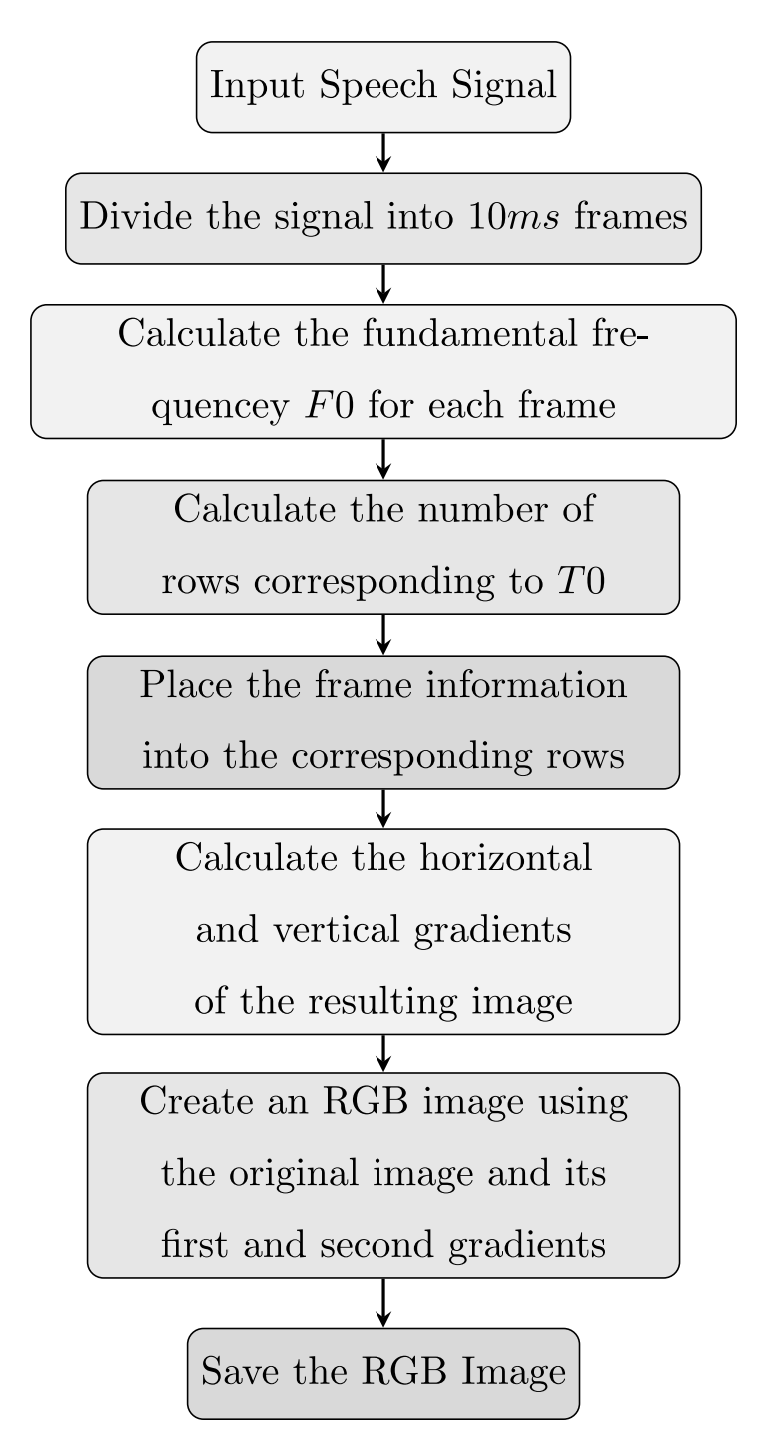
\includegraphics[scale = 0.8]{images/CyTex Procedure Flowchart.png}
        \caption{CyTex transformation process \cite{CyTexRef}}
        \label{cytexFlowchart}
\end{figure}
\subsection{Frame Division}
As speech signals are quasi-periodic, the demonstrate some periodicity, however, also vary in accordance with time. This means that analysing the signal on a global scale is a poor decision as at two distant time-points the signal will likely be drastically different. By dividing the audio signal into smaller width time-frames, as discussed when dealing with the STFT, one is able to capture the temporal evolution of the signal. Smaller time windows also better capture the intonation of speech. This information proves vital for the classification of emotions in this context. As was previously noted, a suitable window length of $10ms$ is chosen for most applications. This strikes a balance of being wide enough to minimise the processing required, while also being small enough to consider the signal as stationary over the time interval. Stationary refers to non-changing frequency and spectral contents over some time interval.

\subsection{Fundamental Frequency via Fourier Transform}
For each window frame $F_{0_n}$ is calculated using the librosa package \cite{mcfee2015librosa}. This uses a modified STFT approach to find the fundamental frequency. Specifications for duration and pitch thresholds must be declared by the user. It may be of interest to make these parameters dynamic or alterable when generalising CyTex to other kinds of data. As one can imagine, the pitch limits set are entirely dependent on the frequency production range of the type of acoustic data being analysed. For human speech contexts, limits of below $1kHz$ are a suitable choice. It is of very important note that the calculation of $F_{0_n}$ is extremely crucial. The benefit of CyTex is that the transform can be conducted purely on the knowledge of $F_{0_n}$. However, the disadvantage of this is that if such a calculation possesses significant error, the entire classification process will dramatically suffer. 

\subsection{Mapping to the Image Domain}
For each frame a fundamental frequency, $F_{0_n}$ is found. The inversion of this is the fundamental period $T_{0_n}$. Each of these periods are to a horizontal row of the CyTex image, having a vertical width of one pixel. This means that the $n^{th}$ row of the image will correspond to the $n^{th}$ fundamental period. The length of an image row is determined by the sampling rate and the minimum frequency allowance specified to the librosa package. The maximum length is provided in equation \ref{max_width_cytex}.  A sampling frequency, $f_s = 16kHz$, is chosen. This is because all humans should speak well within the band of $[0, 8kHz]$ and the upper limit is double to satisfy the Nyquist rate. Zero-padding is applied in cases where the pixel width does not take up the max length. In practical cases the lower frequency limit is set to $40Hz$ and thus the resulting length is $400$ pixels wide.
\begin{align}\label{max_width_cytex}
    S_{T_{max}} &= \dfrac{f_s}{f_{min}} \\ \nonumber
                &= \dfrac{16kHz}{40} \\ \nonumber
                &= 400
\end{align}
 The number of vertical rows is calculated as follows. This height is directly related to the duration of the entire the signal. So, the longer a signal is in the time scale, the taller the resulting CyTex image. 
\begin{align}\label{vert_rows_eqn}
    n = ceil \Big( \dfrac{160 F_{0_n}}{N_{F_{0_n}}} \Big)
\end{align}
Finally, the intensity of the pixels are directly related to the intensity of the signal at that specific point in time. The numerical range of values the pixels can take on is in between 0 and 255 due to the RGB nature of the output image. Pixel intensities at the upper or lower boundaries relate to more intensely felt emotions such as anger or immense joy. The intensity calculation is provided by equation \ref{P_intensity}. Here $S_n$ refers to the speech sampled value at a particular time instant.
\begin{align}\label{P_intensity}
    P_n = round \Big( \dfrac{255 (S_n + 1)}{2} \Big)
\end{align}
A detailed speech to image mapping is illustrated in figure \ref{cytexVis_example}. By working up from the base of the image one can see how a time series signal is mapped to the RGB image domain. 
\begin{figure}
        \centering
        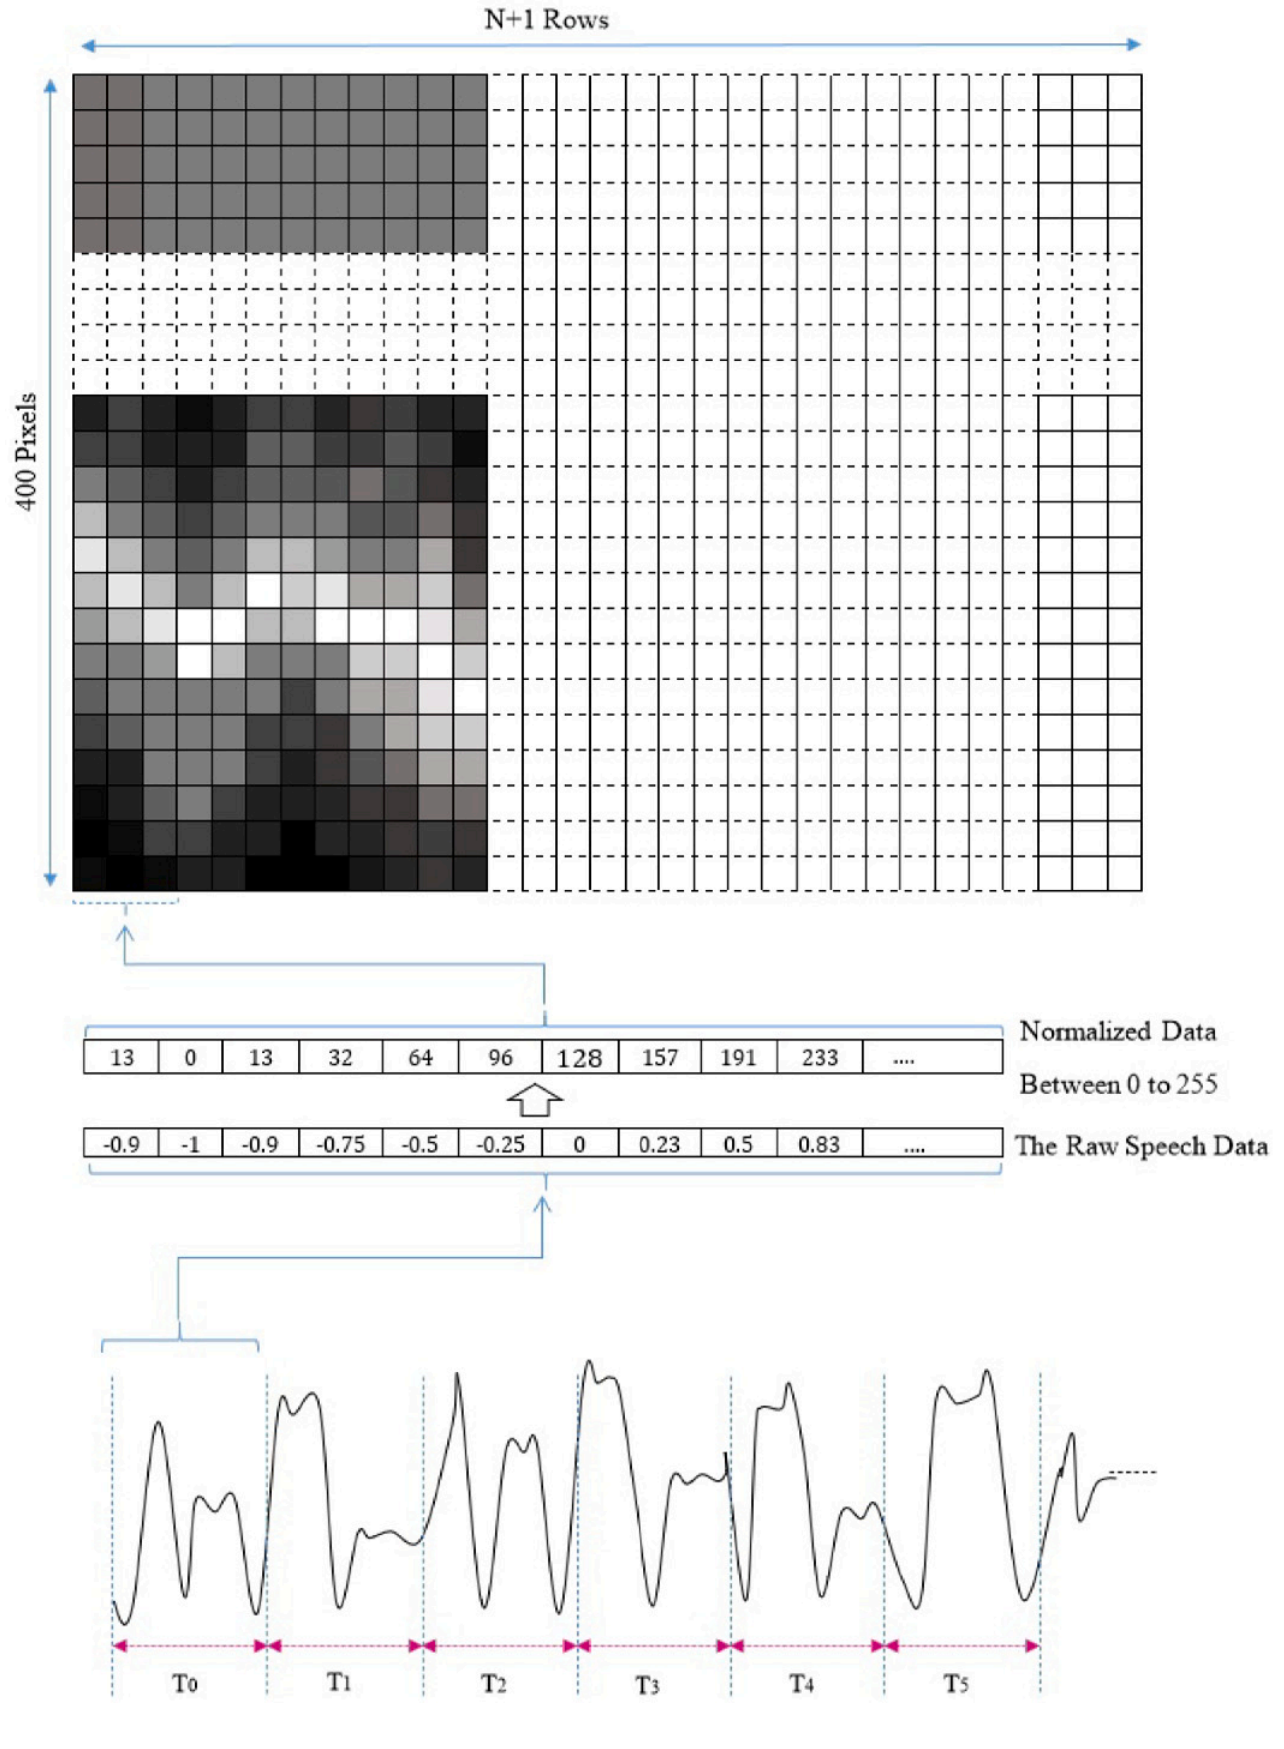
\includegraphics[scale = 1.2]{images/CyTex-diagram.png}
        \caption{CyTex mapping visualized \cite{CyTexRef}}
        \label{cytexVis_example}
\end{figure}

\subsection{RGB Texturing the Image}
Following this, the gradients of the image are calculated. If one was to imagine what these would correspond to in an acoustic sense, one may liken them to the concavity of the function in time. This would be akin to the change in the audio signal over time. For example, is the pitch of the signal trending in an ascending or descending fashion over time. They also apply some form of continuity and interrelation between separate window analysed singals. The results of these calculations are used as the remaining channels of the three channel RGB image. This portion is also another area of interest for innovation. By finding further information about the signal one can increase the dimension of output CyTex objects. This will encode more information in machine network inputs and improve the classification results. 


% SECTION:
% ================================================
\section{Train and Test Databases for SER}
As this genre of task is one of supervised classification, results are dependent on quality labelled data. The databases used to train the model have a drastic impact on the model performance. After all, a model is only as good as the data from which it is constructed. Several types of SER databases exist. However, each pose their own problems. These databases are categorised as Acted, Elicited and Natural \cite{surveyCORE1}.
\begin{description}
\item[Acted (Simulated) Speech:]
Acted datasets, as the name suggests, are entirely fabricated. Actors are employed and will usually be reading text from a script in a professional studio environment. The intention is to act out a certain emotional state whilst reading this script. Due to the controlled nature of this recording process, the signal quality is typically high and requires little audio preprocessing. The construction of an acted database is also simple as it is only limited by the number of actors and budget for their employment. The artificial nature of such a recording process does, however, have its disadvantages. Namely, it is believed that an actor cannot effectively emulate a given emotion in a completely natural way. That is to say that there may exist a disparity between the speech of an actor and speech uttered in a spontaneously emotional way \cite{campbell_2000_databases}. Actor's dialog can be prone to exaggeration and other features that detract from realism. These issues pose problems for the adaptation of learned models to real world data. Having been trained on potentially 'unrealistic' data can massively impact a machine's ability to make correct classifications. 

\item[Natural Speech:] These databases are the most representative of a user's real-world interactions. In this format participants are, mostly, unaware of their recording, (at least in terms of being judged on their emotion). Thus, the emotions expressed are entirely realistic at the time of audio capture. For example, the "Speech Under Simulated and Actual Stress" (SUSAS) Database contains the audio recordings of participants on roller-coasters and in helicopters, among other induced emotional environments, \cite{SUSAS_1997_DB}. While participants may be aware of their own recording, they still demonstrate authentic emotional responses. The drawback of this approach is that there still exists a disparity between these scenarios and everyday situations. In this case, the physical exertion the participant demonstrates is not representative of a typical user's interaction with a machine. There is also significant audio processing to be carried out prior to analysis due to the nature of the recording environment. Due to the nature of recording mostly unaware participants, such a database becomes difficult to construct with any kind of standardised rigor. Legal issues may also arise when considering intellectual property rights and personal confidentiality. Further, deliberately inducing fear and other strong emotions in experiment participants is illegal in many countries \cite{shaver1987emotion}. For these reasons, natural speech emotion databases are often constructed from publicly available audio sources like television and radio. These formats often produce non-ideal audio signals and require some form of preprocessing such as filtering or isolation.

\item[Elicited (Induced) Speech:]
Elicited databases can be viewed as a mixture of the two aforementioned categories. Participants are placed in environments which aim to stimulate specific emotional responses. After the recording process participants self-report the emotions they experienced. This self-reporting as opposed to human labelling is the key differentiating factor between elicited and natural databases. Finally, the aforementioned legal issues which apply to natural speech databases may also apply in this case. 
\end{description}
% --
An important facet of any database used to train the machine learning model is balance. In terms of a classification problem, each output class (emotion) should have roughly the same number of input classes as all other emotions in the training set. However, balance/diversity must also be imposed in terms of other dimensions of the training and test data. For example, the genders of speakers, speaker ages, repetition of phrases using different actors, etc.
Failure to do so will introduce errors into the model like over-fitting for certain types of data and large variance of classification results. This is particularly relevant in the cases of elicited and natural speech databases. Here one must be more selective with the audio used as one no longer has the ability to enforce artificial balance in the dataset. However, The cost of losing balance in the design of speech signals can be compensated by employing a much larger speech library which will contain similar, albeit shorter, acoustic sub-sequences \cite{campbell_2000_databases}.

\subsection{EMODB Database}
The Berlin Emotional Database is an acted emotional speech database spoken entirely in the German language. An acted speech environment was chosen to ensure the controlability and consistency of all elements of the data, apart from manifestations of emotional speech. To remove the bias of a trained actor's emotional exaggeration, roles were advertised openly in the newspaper. From this advertisement 40 people entered the selection phase. An expert panel chose five members of each gender based on their proficiency's in emotional recognisability naturalness of delivery \cite{EMODB_05b_doc}. The ages of participants ranged in between 21 and 35 years of age at the time of recording \cite{EMODB_97}.\\ \\
Choices for dialog were made to minimise the emotional bias the text contained. This can be done via utilising the two following forms of sentences.\\
\textbf{Nonsensical sentences}, which by nature are difficult to associate with any emotions based on the performer's social sensibilities. Unfortunately, the built-in obscurity of such sentences can lead to emotional exaggeration from performers \cite{scherer1981speech}.\\
\textbf{Normal sentences}, which are used so commonly that the performer should be emotionally indifferent to them. These sentences are also simple for actors to rethink in different emotional contexts.\\ \\
\textit{Normal sentences} were chosen for the particular database as "the
use of everyday communication has proved best \cite{scherer1981speech}", due to resembling natural speech when a subject is under emotional stimulation. Ten distinct phrases were spoken and recorded by each actor. Seven distinct emotional states were utilised during the performance process. Each of the phrases and emotions from the dataset are detailed in tables \ref{EMODB_phrase_table} and \ref{EMODB_emo_table}, respectively.
\begin{table}[]
\begin{tabular}{|c|l|l|}
\hline
Code & German Text                            & English Translation                    \\ \hline\hline
a01  & Der Lappen liegt auf dem Eisschrank.   & The tablecloth is lying on the frigde. \\ \hline
a02  & Das will sie am Mittwoch abgeben.      & She will hand it in on Wednesday.      \\ \hline
a04  & Heute abend könnte ich es ihm sagen.   & Tonight I could tell him.              \\ \hline
a05 &
  \begin{tabular}[c]{@{}l@{}}Das schwarze Stück Papier befindet \\ sich da oben neben dem Holzstück.\end{tabular} &
  \begin{tabular}[c]{@{}l@{}}The black sheet of paper is located\\  up there besides the piece of timber.\end{tabular} \\ \hline
a07  & In sieben Stunden wird es soweit sein. & In seven hours it will be.             \\ \hline
b01 &
  \begin{tabular}[c]{@{}l@{}}Was sind denn das für Tüten, die da \\ unter dem Tisch stehen?\end{tabular} &
  \begin{tabular}[c]{@{}l@{}}What about the bags standing \\ there under the table?\end{tabular} \\ \hline
b02 &
  \begin{tabular}[c]{@{}l@{}}Sie haben es gerade hochgetragen und\\  jetzt gehen sie wieder runter.\end{tabular} &
  \begin{tabular}[c]{@{}l@{}}They just carried it upstairs and\\ now they are going down again.\end{tabular} \\ \hline
b03 &
  \begin{tabular}[c]{@{}l@{}}An den Wochenenden bin ich jetzt immer\\  nach Hause gefahren und habe Agnes besucht.\end{tabular} &
  \begin{tabular}[c]{@{}l@{}}Currently at the weekends I always\\ went home and saw Agnes.\end{tabular} \\ \hline
b09 &
  \begin{tabular}[c]{@{}l@{}}Ich will das eben wegbringen und \\ dann mit Karl was trinken gehen.\end{tabular} &
  \begin{tabular}[c]{@{}l@{}}I will just discard this and then\\ go for a drink with Karl.\end{tabular} \\ \hline
b10 &
  \begin{tabular}[c]{@{}l@{}}Die wird auf dem Platz sein,\\ wo wir sie immer hinlegen.\end{tabular} &
  \begin{tabular}[c]{@{}l@{}}It will be in the place where we\\ always store it.\end{tabular} \\ \hline
\end{tabular}
    \caption{EMODB Simulated Phrases \cite{EMODB_97}}
    \label{EMODB_phrase_table}
\end{table}


\begin{table}[]
    \centering
    \begin{tabular}{|llll|}
    \hline
    \multicolumn{2}{|c|}{English}                                    & \multicolumn{2}{c|}{German}               \\ \hline\hline
    \multicolumn{1}{|l|}{Letter} & \multicolumn{1}{l|}{Emotion}      & \multicolumn{1}{l|}{Letter} & Emotion     \\ \hline
    \multicolumn{1}{|l|}{A}      & \multicolumn{1}{l|}{Anger}        & \multicolumn{1}{l|}{W}      & Ärger (Wut) \\ \hline
    \multicolumn{1}{|l|}{B}      & \multicolumn{1}{l|}{Boredom}      & \multicolumn{1}{l|}{L}      & Langeweile  \\ \hline
    \multicolumn{1}{|l|}{D}      & \multicolumn{1}{l|}{Disgust}      & \multicolumn{1}{l|}{E}      & Ekel        \\ \hline
    \multicolumn{1}{|l|}{F}      & \multicolumn{1}{l|}{Anxiety/Fear} & \multicolumn{1}{l|}{A}      & Angst       \\ \hline
    \multicolumn{1}{|l|}{H}      & \multicolumn{1}{l|}{Happiness}    & \multicolumn{1}{l|}{F}      & Freude      \\ \hline
    \multicolumn{1}{|l|}{S}      & \multicolumn{1}{l|}{Sadness}      & \multicolumn{1}{l|}{T}      & Trauer      \\ \hline
    \multicolumn{4}{|c|}{N = Neutral Emotion} \\ \hline
    \end{tabular}
    \caption{Emotions of the EMODB Dataset \cite{EMODB_97}}
    \label{EMODB_emo_table}
\end{table}


Audio was recorded in an anechoic chamber at the Technical University Berlin, sampled at 48kHz and later sampled down at a rate of 16kHz. The audio is of a high quality and requires little to no processing to improve clarity of the acoustic signals. In total there are 700 labelled emotional acoustic signals (7 emotions, 10 actors, 10 unique phrases). As this database is also open to he public it has found immense popularity in the SER research community. 
% It has been chosen as the prime bench-marking database to grade the performance of the results this study seeks to create.


\subsection{RAVDESS Database}
The Ryerson Audio-Visual Database of Emotional Speech and Song (RAVDESS) is another simulated speech dataset, similar to the EMODB dataset. However, this dataset is recorded entirely with English speaking actors from Ontario, Canada. Also unlike EMODB, the dataset also includes facial expression video recordings of actors whilst performing speech and song. This video footage was not analysed for the purposes of this study, however, as the aim is to perform emotional classification purely from audio signals. Only the audio exclusive signals were utilised from this dataset within this project. RAVDESS also, rather uniquely, includes the performance of emotional song. \\ \\
One of the most attractive factors, which has seen the RAVDESS dataset become a standard in SER, is its size. RAVDESS boasts 7356 multi-modal recordings,, consisting of 4320 speech recordings and 3036 song recordings. This is over 10 times the size of the EMODB dataset. Such a large corpus is ideal for machine learning methods. With larger training and testing sets directly improve training and testing results, generally. These clips are composed of a gender balanced cast of 24 professional actors. Actors are tasked with performing at two different emotional intensities, normal and strong, for each of the emotions detailed in table \ref{rav_emo_table}. The incorporation of different intensities is key, as intensity is one of the most salient indicators of emotion \cite{sonnemans1994structure}. 
\begin{table}[]
    \centering
    \begin{tabular}{|c|c|}
    \hline
    Code & Emotion \\ \hline \hline
    01 & neutral \\ \hline
    02 & calm \\ \hline
    03 & happy \\ \hline
    04 & sad \\ \hline
    05 & angry \\ \hline
    06 & fearful \\ \hline
    07 & disgust \\ \hline
    08 & surprised \\ \hline
    \end{tabular}
    \caption{Emotions of RAVDESS \cite{ravdess_dataset_2018}}
    \label{rav_emo_table}
\end{table}
Professional actors are utilised, as for the other datasets, as \cite{EMODB_05b_doc} details that the most identifiable emotional performances are created by actors. Actors were selected from the Toronto, Ontario region of Canada. Interestingly, this region's accent does not prominently exhibit a feature of the Canadian accent known as "Canadian raising" \cite{ravdess_journal}. This phenomena was also avoided via appropriate selection of the stimulus statements. These stimulus statements consisted of two sentences. Firstly, "Kids are talking by the door", and secondly, "Dogs are sitting by the door." These are both examples of \textit{normal sentences}, which the EMODB dataset also makes use of. The studio recording environment is displayed in figure \ref{ravdessstudio}. The complete process of the construction and validation of the RAVDESS dataset is illustrated in figure \ref{ravdessFlowchart}.\\ \\
It is important to note the naming convention of files in the RAVDESS dataset. The filenames are used to distinguish the characteristics of different samples. They are key for separating data points into different classes of emotions, prior to training a deep learning model. Characteristic identifiers are separated by hyphens and are ordered: Modality–Channel–Emotion–Intensity–Statement–Repetition–Actor. Table \ref{rav_code_table} comprehensively highlights the filename identifiers and the characteristic associated with each.
\begin{table}[]
    \centering
    \begin{tabular}{|l|l|}
    \hline
    Identifier & Coding Description of Factor Levels          \\ \hline\hline
    Modality   & 01=Audio-video, 02=Video-only, 03=Audio-only \\ \hline
    Channel    & 01=Speech, 02=Song                           \\ \hline
    Emotion   & \begin{tabular}[c]{@{}l@{}}01=Neutral, 02=Calm, 03=Happy, 04=Sad, 05=Angry,\\ 06=Fearful, 07=Disgust, 08=Surprised\end{tabular} \\ \hline
    Intensity  & 01=Normal, 02=Strong                         \\ \hline
    Statement & \begin{tabular}[c]{@{}l@{}}01="Kids are talking by the door.",\\ 02="Dogs are sitting by the door."\end{tabular}                \\ \hline
    Repetition & 01=First, 02=Second                          \\ \hline
    Actor      & 01=First actor, ..., 24=Twenty-fourth actor  \\ \hline
    \end{tabular}
    \caption{Code Protocol of RAVDESS \cite{ravdess_dataset_2018}}
    \label{rav_code_table}
\end{table}

\begin{figure}
    \centering
    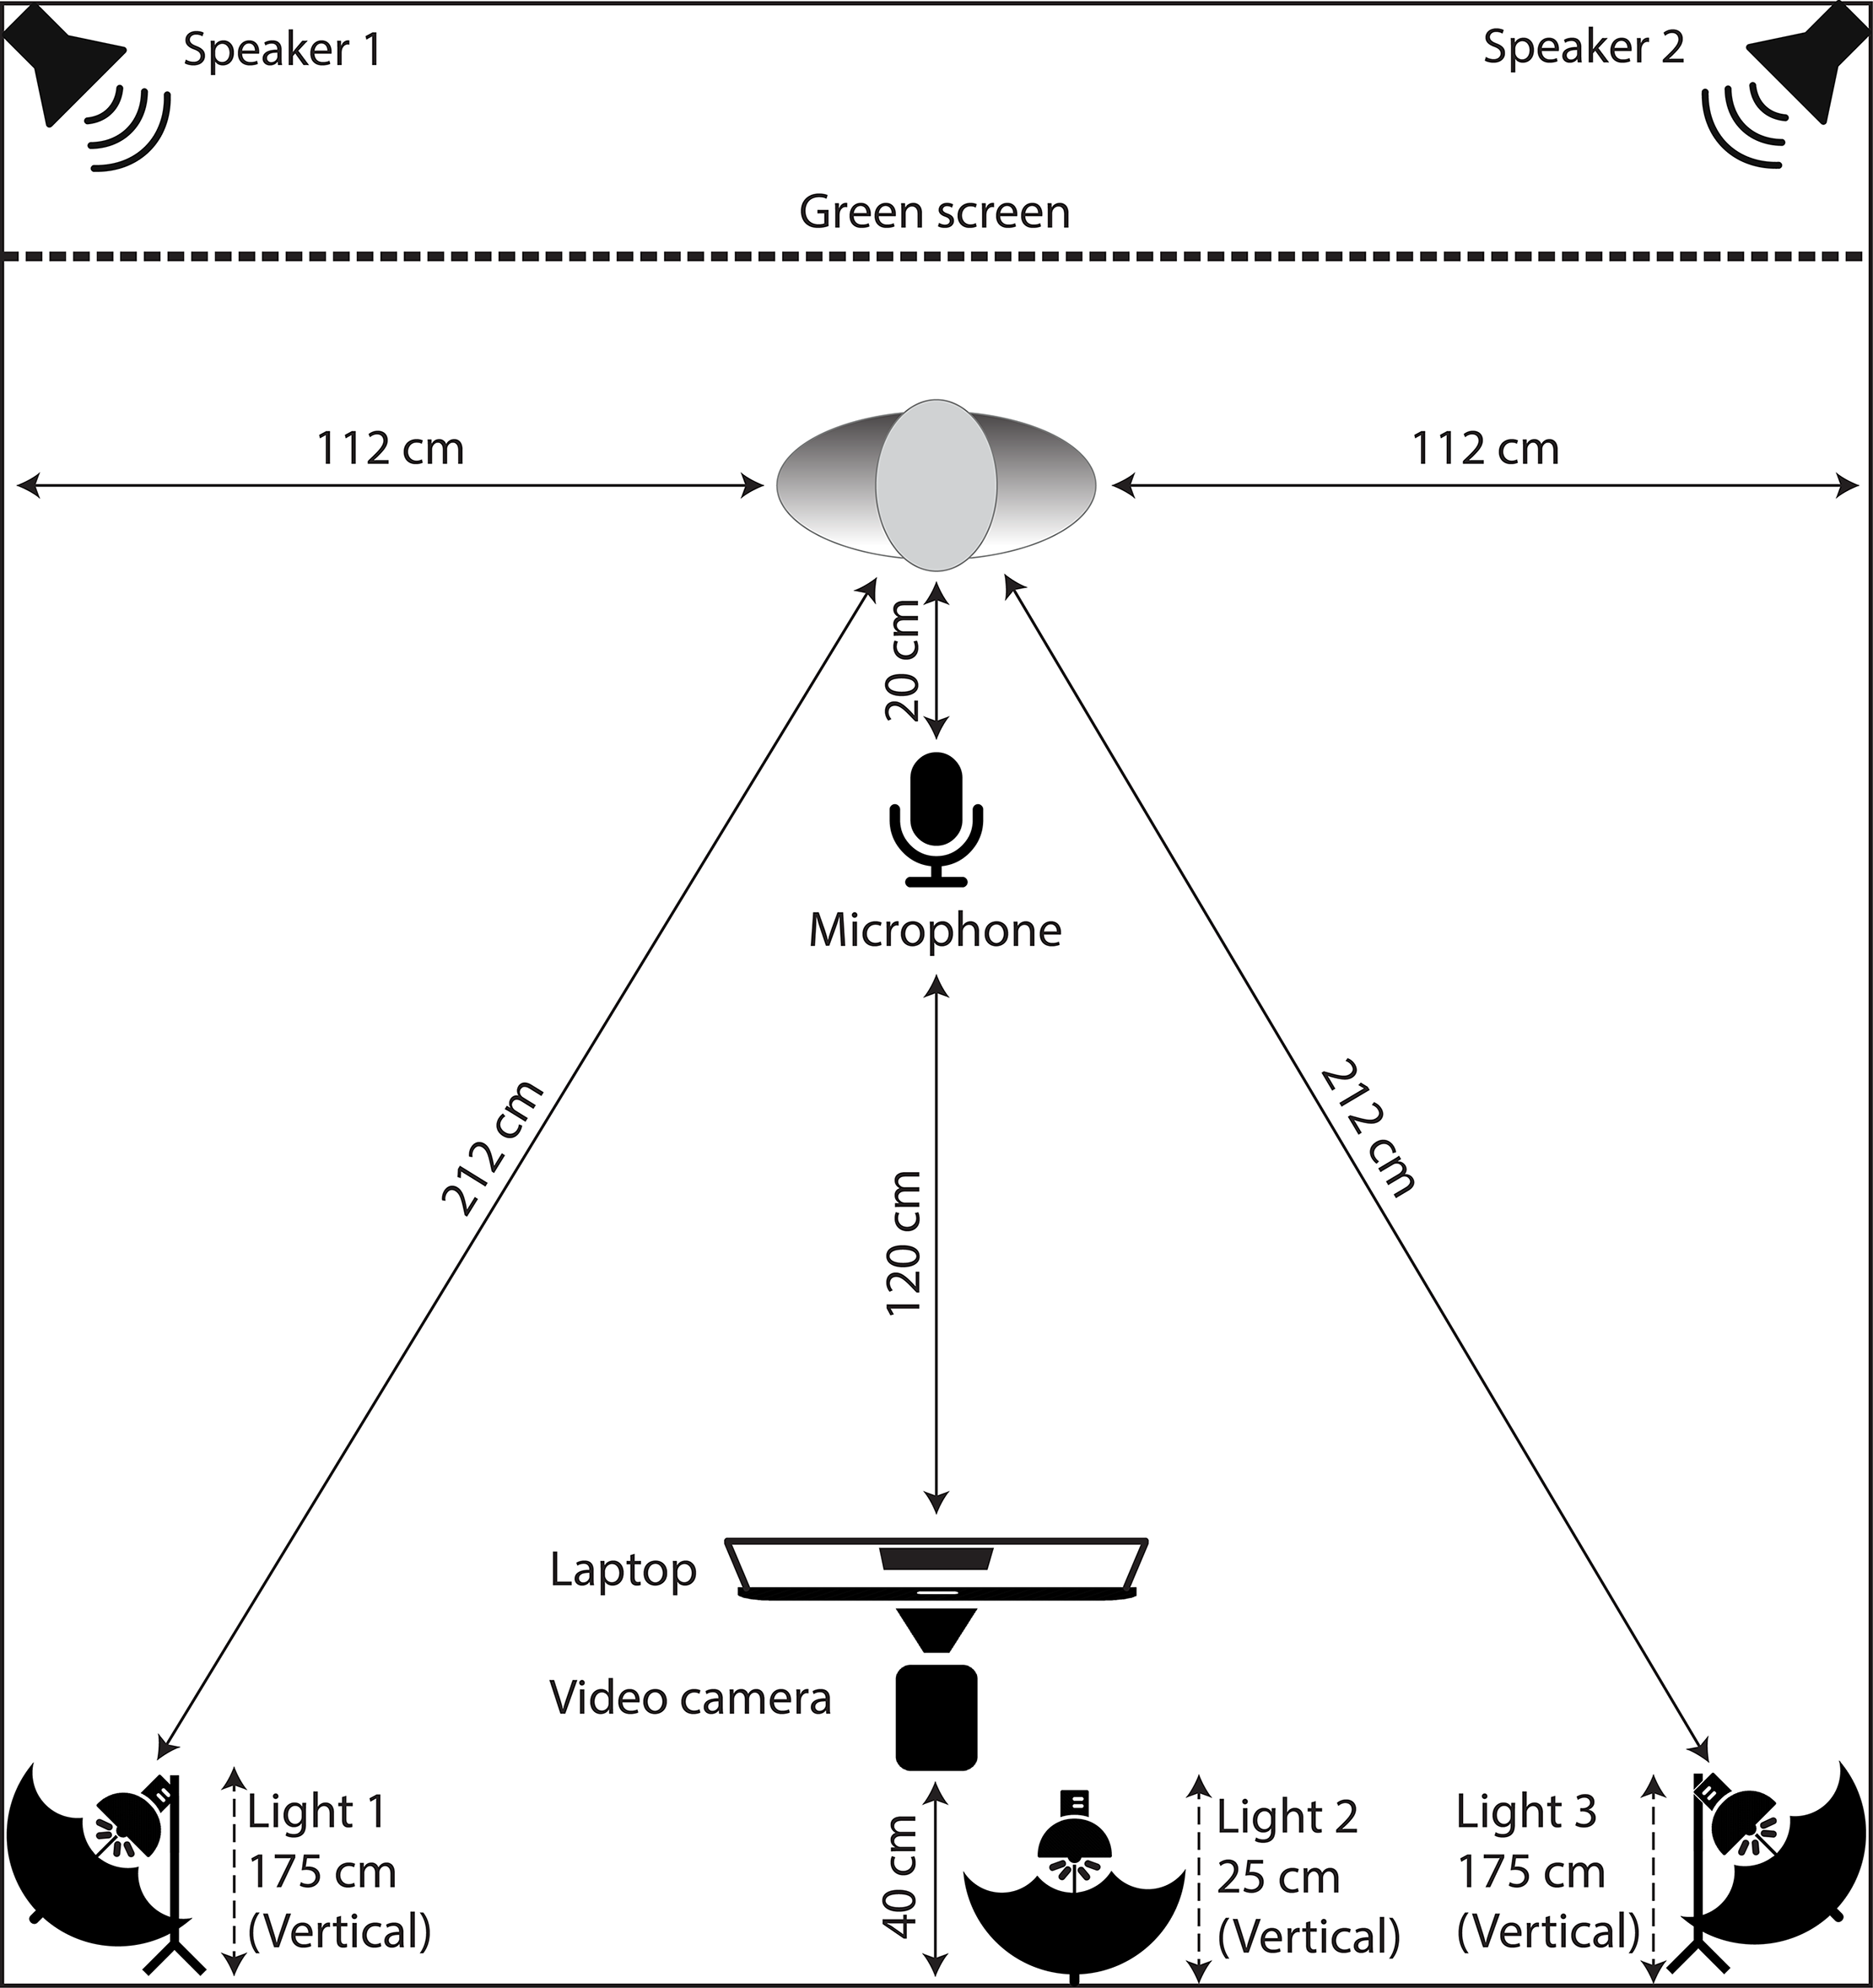
\includegraphics[scale = 0.4]{images/RAVDESS_studioSetup.png}
    \caption{RAVDESS recording environment \cite{ravdess_journal}}
    \label{ravdessstudio}
\end{figure}

\begin{figure}
        \centering
        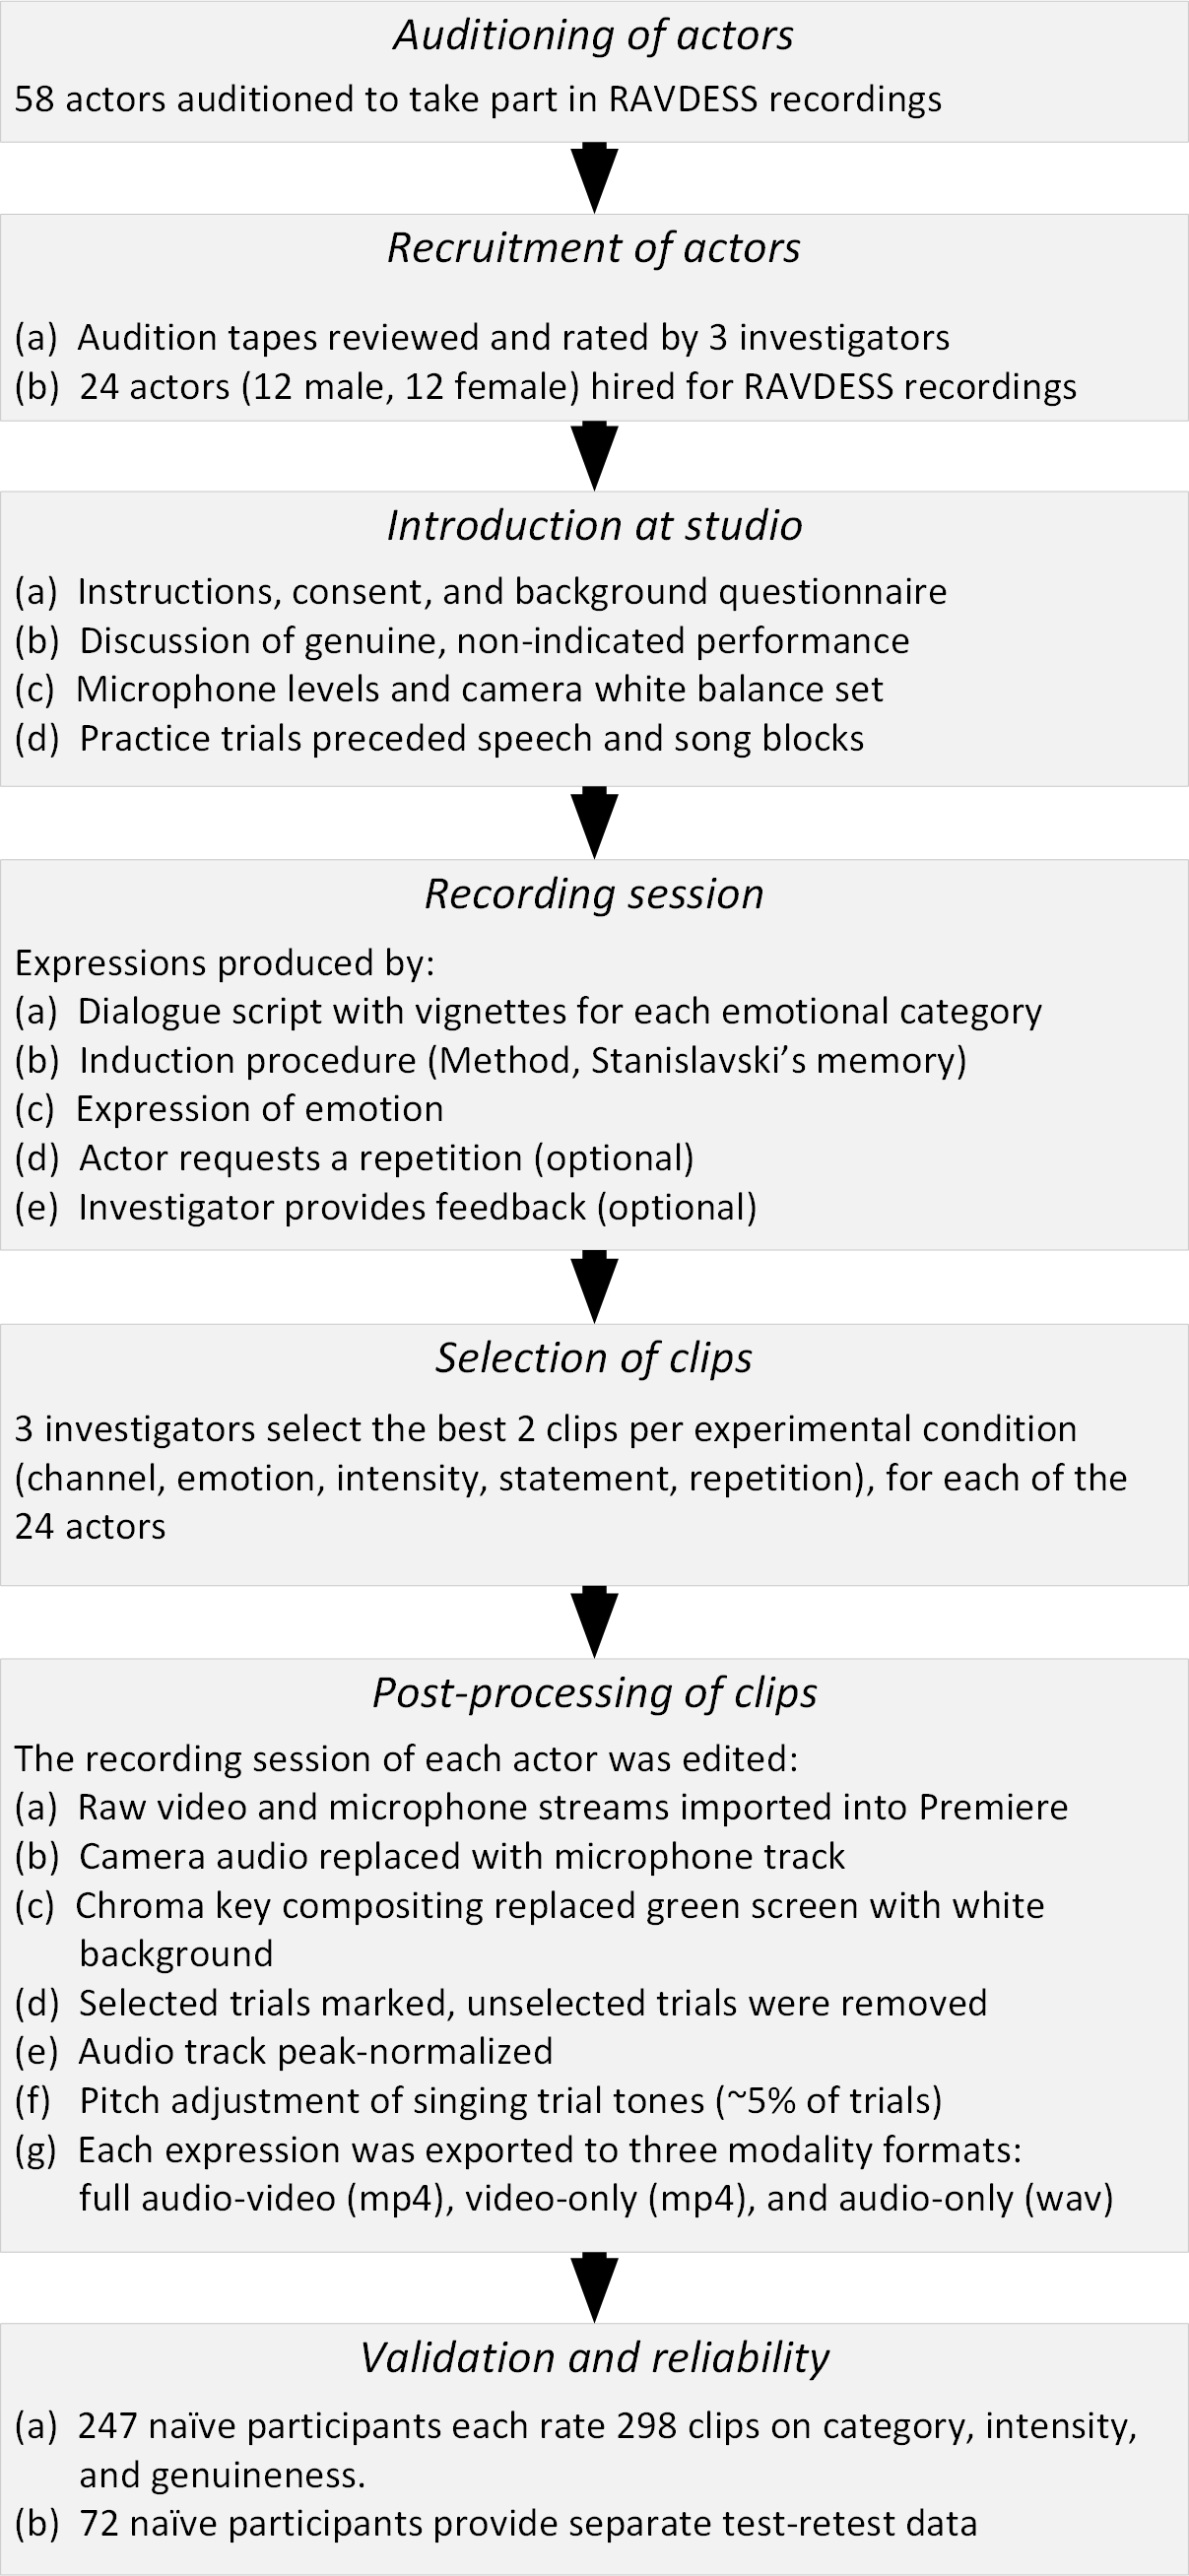
\includegraphics[scale = 1.0]{images/RAVDESS_process.png}
        \caption{RAVDESS construction flowchart \cite{ravdess_journal}}
        \label{ravdessFlowchart}
\end{figure}


\subsection{IEMOCAP Database}
This dataset, while not directly used for the gathering of results in this report, was used in the original CyTex research paper \cite{CyTexRef}. This was motivated by the fact that the RAVDESS dataset had not been previously tested. Instead, the RAVDESS dataset was used.\\ \\
The Interactive Emotional Dyadic Motion Capture (IEMOCAP) Database was constructed is a widely used and accepted benchmark dataset for SER. One of the distinguishing features of this dataset is the wealth of different modalities accessible. Like the RAVDESS, both speech and video are employed. However, modalities like facial motion capture, head angle, head movement, and dialog transcriptions are also available. The dataset was created with the intent to expand research in the areas of gesture and speech relationships, as well as linguistics and communications goals \cite{IEMOCAP_doc}.\\ \\
While the IEMOCAP database is primarily comprised of simulated speech, actors are also given hypothetical scenarios in which their dialog is entirely improvised. This is done with the intent of eliciting emotions from the actor, hence increasing emotional genuineness. In total 10 actors (5 male and female) were used for the recording of this dataset. The spoken language demonstrated throughout is English. Recording was conducted in pairs of actors (dyadic recording sessions). The total accumulated time of all data samples is roughly 12 hours. A relatively standard set of emotions are used in IEMOCAP. This set of emotions are listed in table \ref{iemocap_emo_table}.\\ \\
\begin{table}[]
    \centering
    \begin{tabular}{|c|}
    \hline
    Emotion \\ \hline \hline
    happiness \\ \hline
    anger \\ \hline
    sadness \\ \hline
    neutral \\ \hline
    frustration \\ \hline
    \end{tabular}
    \caption{Emotions of IEMOCAP}
    \label{iemocap_emo_table}
\end{table}
Two different material selection approaches were chosen throughout the recording process. As mentioned prior, improvised scenarios were used to provide some form of induced emotional speech. More conventionally, scripted dialog was exerted from plays was also used, demonstrating simulated speech. This later form offers control over experiment and recording parameters, while the unscripted recordings allow for generalizability to authentic emotions. Each of the play exerts contain verbal interaction between a singular male and female only. These recordings more closely approximate genuine emotion given the greater context of the play \cite{IEMOCAP_doc}. The improvised recordings stemmed from a set list of hypothetical scenarios proposed by \cite{scherer1986experiencing} and detailed in table \ref{iemocap_scenario_table}.
\begin{table}[]
\centering
\begin{tabular}{l|l|l|}
\cline{2-3}
 & Subject 1 (with markers) & Subject 2 (without markers) \\ \hline\hline
\multicolumn{1}{|l|}{1} & \begin{tabular}[c]{@{}l@{}}(Fru) The subject is at the Department \\ of Motor Vehicles (DMV) and he/she is\\ being sent back after standing in line for\\ an hour for not having the right forms of IDs.\end{tabular} & \begin{tabular}[c]{@{}l@{}}(Ang) The subject works\\ at DMV. He/she rejects\\ the application.\end{tabular} \\ \hline
\multicolumn{1}{|l|}{2} & \begin{tabular}[c]{@{}l@{}}(Sad) The subject, a new parent, was called\\ to enroll in the army in a foreign country. \\ He/she has to separate from his/her spouse\\ for more than 1 year.\end{tabular} & \begin{tabular}[c]{@{}l@{}}(Sad) The subject is\\ his/her spouse and is \\ extremely sad for the\\ separation.\end{tabular} \\ \hline
\multicolumn{1}{|l|}{3} & \begin{tabular}[c]{@{}l@{}}(Hap) The subject is telling his/her friend \\ that he/she is getting married.\end{tabular} & \begin{tabular}[c]{@{}l@{}}(Hap) The subject is\\ very happy and wants\\ to know all the details\\ of the proposal. He/she\\ also wants to know the\\ date of the wedding.\end{tabular} \\ \hline
\multicolumn{1}{|l|}{4} & \begin{tabular}[c]{@{}l@{}}(Fru) The subject is unemployed and \\ he/she has spent the last 3 years looking\\ for work in his/her area. He/she is \\ losing hope.\end{tabular} & \begin{tabular}[c]{@{}l@{}}(Neu) The subject is \\ trying to encourage\\ his/her friend.\end{tabular} \\ \hline
\multicolumn{1}{|l|}{5} & \begin{tabular}[c]{@{}l@{}}(Ang) The subject is furious, because\\ the airline lost his/her baggage and \\ he/she will receive only \$50 (for a \\ bag that cost over \$150 and has lots \\ of important things).\end{tabular} & \begin{tabular}[c]{@{}l@{}}(Neu) The subject works\\  for the airline. He/she tries\\ to calm the customer.\end{tabular} \\ \hline
\multicolumn{1}{|l|}{6} & \begin{tabular}[c]{@{}l@{}}(Sad) The subject is sad because a\\ close friend died. He had cancer that\\ was detected a year before his death.\end{tabular} & \begin{tabular}[c]{@{}l@{}}(Neu) The subject is trying\\ to support his friend in this\\ difficult moment.\end{tabular} \\ \hline
\multicolumn{1}{|l|}{7} & \begin{tabular}[c]{@{}l@{}}(Hap) The subject has been accepted\\  at USC. He/she is telling this to \\ his/her best friend.\end{tabular} & \begin{tabular}[c]{@{}l@{}}(Hap) The subject is very\\ happy and wants to know\\ the details (major, scholarship).\\ He/she is also happy because \\ he/she will stay in LA so\\ they will be together.\end{tabular} \\ \hline
\multicolumn{1}{|l|}{8} & \begin{tabular}[c]{@{}l@{}}(Neu) He/she is trying to change\\ the mood of the customer and\\ solve the problem.\end{tabular} & \begin{tabular}[c]{@{}l@{}}(Ang) After 30 min talking\\ with a machine, he/she is\\ transferred to an operator.\\ He/she expresses his/her \\ frustration, but, finally, he/she\\ changes his/her attitude.\end{tabular} \\ \hline
\end{tabular}
    \caption{Scenarios of IEMOCAP \cite{IEMOCAP_doc}}
    \label{iemocap_scenario_table}
\end{table}
IEMOCAP audio was recorded using a dual microphone setup, (one microphone per actor). Audio was sampled at a frequency of $48kHz$. To prioritize depth of emotion it was required that the two interacting actors were visible to each other. Camera and microphone equipment was positioned to accommodate this.

% SECTION:
% ================================================
\section{Deep Learning Fundamentals}
This section details the fundamental concepts necessary for understanding and applying methods of deep learning in the context of this project. Beginning with motivations of deep learning and traversing theoretical key concepts. One should note, however, that this review is by no means comprehensive. This section merely addresses the required material for understanding subsequent strategies and results of this report.\\ \\

\subsection{The Motivation For Deep Learning}
Problems in the domain of Artificial Intelligence (AI) are generally solved by generating an appropriate set of features to describe trends in a dataset. These features are input into a simple machine learning algorithm. Having analysed these features, the machine learning model can use this information to predict, classify, or make any number of assessments on a dataset. However, it may not be apparent which features best inform an algorithm, or which may be easily extracted. This introduces the concept of \textit{representation learning}. Representation learning utilises machine learning to not only learn patterns in data, (mapping features to outputs), but to learn the very features as well. \textit{Deep Learning} then refers to a sub-branch of representation learning in which complex features of a dataset are created hierarchically from simpler features. An example highlighting the development of complex features based upon simpler variants is illustrated in figure \ref{DL_feature_fig}. The need for deep learning comes about when finding complex features becomes as, or more, challenging than the initial machine learning problem one was trying to solve. One of the key advantages of deep learning is that the more data a model sees, the more complicated features it can build from simpler ones, improving performance. Another asset is the elimination of feature design. The user need not inform the computer of which features are important to determine an output, as the model will learn this itself through the training procedure.
\begin{figure}
        \centering
        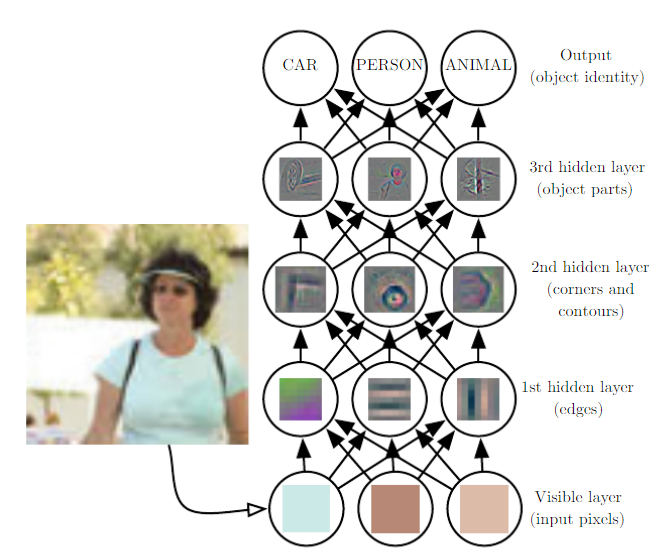
\includegraphics[scale = 0.7]{images/DL_features_figure.png}
        \caption{Deep learning feature generation \cite{Goodfellow-et-al-2016}}
        \label{DL_feature_fig}
\end{figure}

\subsection{Machine Learning - Key Concepts}
\subsubsection{Components of Learning}
The phrase 'Machine Learning' consists of two fundamental components we must understand. Where a machine simply refers to a computer, learning is defined more rigorously. To define learning we first introduce three concepts; a task (\textit{T}), performance measure (\textit{P}), and experience (\textit{E}).\\ \\
Firstly, a task \textit{T} is some action or process we wish to perform. Popular examples in contemporary literature include classification, anomaly detection, and regression. Initially, the computer may have no way of executing a process to complete some task. This is where experience \textit{E} enters. Experience refers to the scrutiny of a dataset and the machines interaction with the dataset during this process. This study approaches experience from a \textit{supervised} perspective. That is to say that a supervised learning algorithm experiences the dataset. In this setting example data \textbf{x} is associated with some target value \textbf{y}. The experience of the machine is used to inform the estimation of $p(y|x)$. In other words, finding a relating mapping between an input and provided output. Another setting, not discussed in this work, is that of \textit{unsupervised learning}. Here \textbf{x} is given, however no corresponding output \textbf{y} will be provided to the machine. The machine instead attempts to learn the underlying probability distributions of groups of example data. Finally, the performance measure \textit{P} is a user defined metric which attempts to grade how well an algorithm performs at a given task \textit{T}. The most obvious grading for many models is some indication of accuracy, expressed as a ratio of correct predictions to total predictions made.

\subsubsection{Defining Learning}
Having defined the building blocks of learning, we may now formally define learning by the definition provided by \cite{mitchell_97_ML}. Mitchell poses, “A computer program is said to learn from experience \textit{E} with respect to some class of tasks \textit{T} and performance measure \textit{P}, if its performance at tasks in \textit{T}, as measured by \textit{P}, improves with experience \textit{E}.”

\subsubsection{Generalization and Model Fitting}
Another concept at the core of machine learning is that of \textbf{Generalization}. This refers to model performance graded on data inputs which do not belong to the training set used to learn the model. Generalization is important as any model is essentially useless if it cannot perform its intended function on input data it has not seen before. In the pursuit of attaining sufficient model generalization, one must be weary of two undesirable phenomena, \textit{underfitting} and \textit{overfitting}. Underfitting implies that the model has not sufficiently been trained and cannot extract enough meaning from the training data to perform its intended task. Overfitting, conversely, refers to giving the model too much exposure to training data. In this case, a model may be memorizing training data, as opposed to intelligently identifying prominent features and characteristics of the data. This typically results in large training accuracy and poor generalization (low test and validation accuracy). Both of the phenomena can be visualized in figure \ref{biasVarTrade}. Here the capacity informally refers to a model's ability to broadly fit many functions \cite{Goodfellow-et-al-2016}. It can be seen that as capacity increases the training error, (approximately indicated by bias), decreases. However, the generalization error after some point begins to increase. This indicates that there is some optimal point at which one should stop training a machine learning model to optimise generalizability.
\begin{figure}
    \centering
    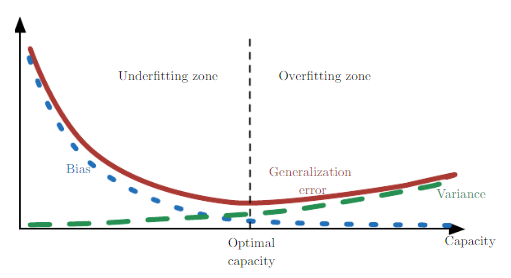
\includegraphics[scale = 1.0]{images/BiasVarTradeOff_Fig.png}
    \caption{Bias variance trade-off and model fitting \cite{Goodfellow-et-al-2016}}
    \label{biasVarTrade}
\end{figure}

\subsubsection{Bias and Variance}
In defining bias and variance, we first define a point estimator of some parameter $\pmb{\theta}$ as in equation \ref{pointEst_eq}. Here each $\pmb{x}$ is an independent and identically distributed (i.i.d.) data point.
\begin{equation}
    \hat{\pmb{\theta}}_m = g(\pmb{x}^{(1)}, ..., \pmb{x}^{(m)})
    \label{pointEst_eq}
\end{equation}
Bias may then be defined by equation \ref{bias_eq}.
\begin{equation}
    bias(\hat{\pmb{\theta}}_m) = \mathrm{E}(\hat{\pmb{\theta}}_m) - \pmb{\theta}
    \label{bias_eq}
\end{equation}
That is to say the bias is given by the difference between the expected value of the point estimator of some parameter and the true underlying value of that parameter. An estimator is called unbiased if, in this case, equation \ref{bias_eq} equates to zero. In a machine learning context, bias gives an indication of how well a model understands the data and its characteristics within a training set. It measures the 'distance' (or error) between a prediction and some actual value. For this reason it is optimal to minimise bias , although only to a point (refer to figure \ref{biasVarTrade}).\\ \\
One must also consider the variance of an estimator. Variance indicates how sensitive a model is to perturbations within the training set. The variance of an estimator is defined in terms of conventional statistical variance, see equation \ref{var_eq}.
\begin{equation}
    Var(\hat{\theta})
    \label{var_eq}
\end{equation}
As is noted above, variance gives indication of a model's performance on unseen data. For this reason the variance is related to model generalizability. By referring to figure \ref{biasVarTrade}, one may note a compromise that must be made between suitably low bias and variance. This concept is know as the \textbf{bias variance trade-off}. In other words, improvements in training accuracy beyond a certain point sacrifice the extent to which a model can generalize. In this study the trade-off is handled via implementation of cross-validation. 

\subsubsection{Cross-Validation}
A typical split of data involves using $80\%$ of a dataset to create a training set and the remaining $20\%$ to create a test set. One can imagine the motivation of these choices, as a model needs to be exposed to as much data as possible to learn defining characteristics of a dataset. However, a sufficiently large subset must remain for testing to any kind of meaningful results. For smaller datasets, division of the net dataset into train and test sets can introduce uncertainty into the test results of a model. A small test set is akin to an insufficient sample that does not accurately represent the complete dataset. For this reason, along with the ubiquity of smaller than ideal datasets, alternate methods of determining test error performance have been developed.\\ \\
Of particular interest to this study is the method of \textit{k-fold cross validation}. This method partitions datasets into random training and test sets  and executes the training process. After this is complete the training process begins again, however, a different partitioning of the dataset is used to construct the train and test subsets. The name of this method comes from the splitting of the data in subset creation. Data is split into \textit{k} partitions containing no overlapping elements. Of these \textit{k} sets, one will be used as the test set and the remainder will be used for training. Following this, the test set will be iterated to the next partition of data and training will be commenced upon the remaining subsets once more (now including the test set from the previous iteration). This process is executed \textit{k} times and the results of each trial are stored and then averaged.

\subsection{The Classification Problem}
% \subsubsection{Defining Classification}
Classification is the basis of many interesting modern artificial intelligence applications. Be it object recognition employed in driverless cars, or medical diagnosis from particular medical imaging datasets.\\ \\
This task involves specification of an input in terms of it belonging to some group. Each of these groups may be referred to as \textit{classes} or \textit{targets}. A model is trained to develop some mapping function which takes an input and maps it to the most probable class that said input belongs to. This mapping function is notated as $f: \mathbb{R}^n \rightarrow \{1, ..., k\}$ for $k$ number of classes. Outputs may vary depending on the construction of the model and type of problem. In the context of this thesis the probability of a particular input belonging to each of the possible emotional classes is used. The maximum is taken of this output to determine the emotional class with the highest probability for the corresponding input.
% \subsubsection{Outputs Using Softmax}
% Get infor from 6.2.2.3 in deep learning (Ian Goodfellow)

% \subsection{Regularization - Methods of Generalization}
% "Regularization is any modification we make to a learning algorithm that is intended to reduce its generalization error but not its training error", \cite{Goodfellow-et-al-2016}.
% \subsubsection{Dataset Augmentation}
% \subsubsection{Training and Early Stoppage}
% \subsubsection{Dropout}

% \subsection{Model Optimization}
% % TIME PERMITTING:
% % \subsubsection{Minibatch Stochastic Optimization}
% \subsubsection{Neural Network Optimization Difficulties}
% % refer to section 8.2
% % TIME PERMITTING:
% % \subsubsection{Parameter Initialization}
% \subsubsection{Stochastic Gradient Descent}
% \subsubsection{ADAM Stochastic Optimization}
% % discussed in textbook but printed paper is main source! Adaptive learning rate method.
% \subsubsection{Batch Normalization}
% refer to printed batch norm academic paper, textbook also discusses.

\subsection{Convolutional Neural Networks}
Convolutional Neural Networks (CNNs) are networks proficient in grid based data processing and analysis. One prominent example is that of an image. An image is a grid consisting of pixels. For some time CNNs have been very popular due to their high performance and ease of production, given many open source tools and packages exist to aid in their construction. 

\subsubsection{Convolution}
Convolution can be defined in terms of two functions in time, $f(t)$ and $h(t)$. The convolution of these two functions is shown in equation \ref{convolution_eq}.
\begin{equation}
    f(t) * h(t) = \int f(\tau)h(t-\tau) d\tau
    \label{convolution_eq}
\end{equation}
The operation of convolution can also be thought of graphically. The function $h$ is flipped about the y-axis and progressively shifted to the right as the $t$ parameter increases. As this function is shifted, the integral of the multiplied functions is calculated. In equation \ref{convolution_eq}, $f$ may be referred to as the input and $h$ is the kernel or filter. The output of this operation constitutes the interaction between $f$ and $h$ (the input and some filter). This output may be known as the feature map.\\ \\
Due to the nature of signal processing and machine learning taking place in a digital setting, it make sense to discretize this process. Just as was done for in the continuous case, we define discrete time convolution as in equation \ref{disc_conv_eq}.
\begin{equation}
    f[k]*h[k] = \sum^{\infty}_{m=-\infty} f[m]h[k-m]
    \label{disc_conv_eq}
\end{equation}
One may note that the graphical explanation for continuous time convolution still holds in this case. The key difference in discrete time is that the integral of the multiplied functions is no longer calculated. Now, the summation of all multiplied overlapping discrete instances are calculated. 

\subsubsection{Convolution in the Image Domain}
In image processing, the input $f$ will be a tensor representing the input image. The filter $h$ will be some arbitrarily sized tensor of values chosen to appropriately scale the input under convolution. We will label the input image $I$ and the filter (or kernel) as $K$, following the conventions set in \cite{Goodfellow-et-al-2016}. Both of these objects are two-dimensional. The convolution of these objects is defined by equation \ref{2d_conv_eq}.
\begin{equation}
    (I*K)(i, j) = \sum_m\sum_n I(m,n)K(i-m, j-n)
    \label{2d_conv_eq}
\end{equation}
As the filter is now in two-dimensional space, the graphical explanation must be altered slightly. Instead of 'flipping' the filter about the y-axis, as was performed in the on-dimensional case, we must flip the filter about two sets of axes. By flipping the filter about x and y, this is the same as taking the 2-D array and rotating it $180^\circ$ counter clockwise. The filter/kernel is the slid across the two-dimensional image and each overlapping pixel value is multiplied and summed.

\subsubsection{Why CNNs Matter}
The usefulness of this operation lies in a filter's ability to extract features from an input. For example, if the input is a 2-dimensional image, by sliding and convoluting some filter over the image, many features may be extracted. Initially the filtering effect may make edges more prominent and allow the learning algorithm to better detect the edges of objects.\\ \\
Another advantage of using these networks is by restricting the type of interactions between outputs and inputs in convolutional layers. Since the kernel is smaller than an input image, when sliding it over we can detect things in smaller regions. This also results in more efficient computation than matrix multiplication based methods. These kinds of interactions are referred to as \textit{sparse interactions}.\\ \\
Unlike traditional neural networks, CNNs also offer shared parameters. By using shared parameters, less parameters overall need be learned, reducing the net required storage for the learned model.

% \subsubsection{Pooling}


% SECTION:
% ================================================
\section{Transfer Learning - Economic Model Building}
Transfer Learning refers to the process of re-purposing pre-trained deep learning models. These models are initially trained for some problem, and later applied to an adjacent task. In doing so, one can leverage the power of the initial model and save time and computational effort. This process may also improve generalization of the final model. In essence, transfer learning utilises powerful models as starting points to extend upon. 

\subsection{Transfer Learning Basics}
Strategies of machine learning typically employ a training dataset which is used to teach a model patterns in the data. Validation of the learnt model is performed on a test set. Both of these datasets usually have the same feature space and data distribution. If this is not the case, prediction performance can depreciate \cite{SHIMODAIRA2000}. Transfer learning passes on information, which has already been learnt by a model, to improve another model in a related domain. This approach is necessary when training data is hard to obtain, or its size is insufficient, (as is the case for many emotional audio datasets). SER has historically been a smaller research field of interest and, as has previously been noted, is a lot younger than other machine learning fields. This has caused datasets to have limited access, limited size, or be largely/entirely unlabelled. As one can imagine, because emotion is perceived subjectively by humans, labelling emotional speech data is ill-advised. For these reasons, the employment of transfer learning is hugely beneficial for SER tasks which are solved in the image domain.\\ \\
\textbf{Defining Transfer Learning}\\
To formally define transfer learning, this report uses the conventions in notation and definition of the prominent surveys \cite{IEEE_TL_Survey} and \cite{2016transfer_survey}. Before defining transfer learning, we must first define its constituents. A \textit{domain} $\mathcal{D}$ has some feature space $\mathcal{X}$ and a marginal probability distribution $P(X)$, with the feature space $\mathcal{X}$ containing all feature vectors for a given learning sample $X = \{ x_1, ..., x_n \}$. The domain can be notated $\mathcal{D} = \{ \mathcal{X}, P(X) \}$.\\
A \textit{task} $\mathcal{T}$ is notated as $\mathcal{T} = \{ \mathcal{Y}, f(\cdot) \}$. Here, $\mathcal{Y}$ is the \textit{label space}, and $f(\cdot)$ is an objective predictive function. The objective predictive function is not known, however, by observing trends in training data, a suitable $f(\cdot)$ can be learned such that a label $y$ from instance $x$ can be predicted. In this training data, each $x_i$ is associated with a corresponding $y_i$. Thus, the objective predictive function can be written in conditional probabilistic terms as $f(x) = P(y|x)$.\\
Finally, we can define two different types of associated domains and tasks in the context of transfer learning. The source domain $\mathcal{D}_S = \{ \mathcal{X}_S, P(X_S) \}$ and source task $\mathcal{T}_S = \{ \mathcal{Y_S}, f_S(\cdot) \}$ both stem from some machine learning problem. In this paper's context, the source domain is images and the source task is the classification of objects in those images. The target domain $\mathcal{D}_T = \{ \mathcal{X}_T, P(X_T) \}$ and target task $\mathcal{T}_T = \{ \mathcal{Y_T}, f_T(\cdot) \}$ are also related to some machine learning problem, which may share similarities with the source problem. Again, in the context of this study, the target domain is images. However, the target task is emotional classification. Finally, we define transfer learning as the following.\\ \\
\textit{Given a source domain and learning task, along with target equivalents $\mathcal{D}_S$, $\mathcal{T}_S$, $\mathcal{D}_T$ and $\mathcal{T}_T$, respectively,  transfer learning aims to improve the learning ability of $f_T(\cdot)$ using previously learnt knowledge in $\mathcal{D}_S$ and $\mathcal{T}_S$. In this case either $\mathcal{T}_S \neq \mathcal{T}_T$, or $\mathcal{D}_S \neq \mathcal{D}_T$} \cite{IEEE_TL_Survey}.\\ \\


% WONT HAVE TIME TO INCLUDE :(
% \subsection{Translation of Deep Learning Features}
% \textbf{***Get info from transferable features paper!}\\
% \cite{yosinski2014transferable}\\


% \subsection{CyTex Enabling Transfer Learning}
%  The power of transfer learning is unlocked through mappings like the CyTex transform.


% TALK ABOUT TRANSFER LEARNING. Two different resources to use here. A gentle introduction webpage in bookmarks + use survey, first few pages with definitions.

